\documentclass[../main.tex]{subfiles}
\begin{document}

\section[Корректность задачи Коши]{Понятие о корректности задачи Коши. Пример Адамара некорректной задачи (задача Коши для уравнения Лапласа).}
% Затехал: Рязанов Андрей

\Subsection{Понятие о корректности}

Рассмотрим абстрактную дифференциальную задачу:
\begin{equation}
\label{eq::2::diff}
\tag{*}
\begin{cases} L\, u(\vec{x}) = f(\vec{x}),\ &\vec{x} \in \Omega \subseteq \R^n  \\
B_j\, u(\vec{x}) = g_j(\vec{x}),\ &\vec{x}\in \Gamma \subset \overline{\Omega},\quad j = 1, \ldots, m
\end{cases}
\end{equation}
$L\;\, = L(\vec{x}, \partial)\;\,$ --- линейный дифференциальный оператор порядка $p$\\
$B_j = B_j(\vec{x}, \partial)$ --- конечное семейство линейных дифференциальных операторов на $\Gamma \subset \bar{\Omega}$

\begin{center}
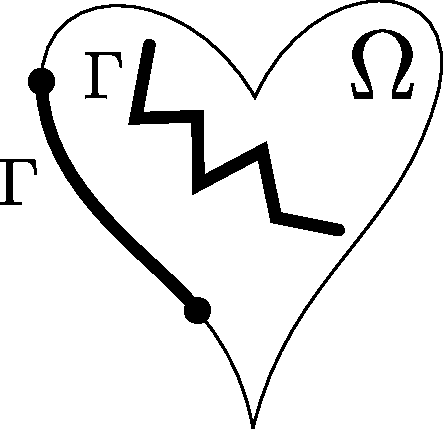
\includegraphics[width=0.15\textwidth]{pic 4_1.pdf}
\end{center}

\begin{definition}
Пусть $F(\Omega)$ и $U(\Omega)$ -- линейные нормированные пространства функций (ЛНП) на $\Omega$, \; $G_1(\Gamma),\dots, G_m(\Gamma)$ -- ЛНП на $\Gamma$.

Тогда если $\ \forall\: f(\vec{x}) \in F(\Omega), \Forall g_j(\vec{x}) \in G_j(\Gamma)$ решение краевой задачи \eqref{eq::2::diff} существует, единственно в $U(\Omega)$ и для него справедлива оценка
\begin{equation}
    \norm*{u}_{U(\Omega)} \leq C\norm*{f}_{F(\Omega)} + \sum\limits_{j=1}^{m}C_j\norm*{g_j}_{G_j(\Gamma)}
\label{eq::2::neq}
\tag{**}
\end{equation}
то {\bf задача корректна по отношению к выбранному набору пространств.}
\end{definition}

\begin{remark}
    Часто говорят, что решение корректной задачи должно непрерывно зависеть от начальных данных. Но в определении лектора, которое приведено выше, вместо непрерывности по начальным данным требуется ограниченность. Так тоже правильно, потому что задача линейна, а линейные операторы непрерывны тогда и только тогда, когда они ограничены.
\end{remark}

\imaginarySubsection{Пример Адамара}
\begin{example}[Адамара]
Рассмотрим задачу Коши для уравнения Лапласа:

$\begin{cases} u_{xx}+u_{yy} = 0 \\
\eval{u}_{y=0} = u_0(x) = e^{-\sqrt{n}}\cos{nx} \text{ --- равномерно стремится к 0 вместе со своими производными} \\
u_y|_{y=0} = u_1(x) \equiv 0
\end{cases}$

При $u_0(x) \equiv 0$ решением будет $u(x,y) \equiv 0$. 

Если задача корректна, то при $n \rightarrow \infty$ решения должны (равномерно?) стремиться к 0.

Функции $u_n=e^{-\sqrt{n}}\cos{nx}\ch{ny}$ -- решения.

Но $u_n(0, y^*) = e^{-\sqrt{n}}\ch{ny^*} > \frac1{2}e^{-\sqrt{n}}e^{ny^*} \rightarrow \infty$

Неравенство \eqref{eq::2::neq} не выполнено.
\end{example}
\end{document}